\section{Use Cases}
\label{sec:use_cases}

This section will present the use cases for the system, divided into four actors: system owner, organizer, validator, and user. All of them have similar use case, the authenticate use case, which is responsible for authenticating the users in the system.
On the Subsection \ref{subsec:system_owner_use_cases} we have the use cases for the system owner, where it mentions the management of the system settings and the control of the organizers that have access.
On the Subsection \ref{subsec:organizer_use_cases} we have the use cases for the organizer that mention the creation and management of the events, along with the control of the validators for the event.
On the Subsection \ref{subsec:validator_use_cases} we have the use cases for the validator, and the only thing he can do is to validate the users' tickets.
Lastly, on the Subsection \ref{subsec:user_use_cases} we have the use cases for the common user, like the purchase, gift, refund and resell of tickets.

\subsection{System owner use cases}
\label{subsec:system_owner_use_cases}

\begin{figure}[H]
    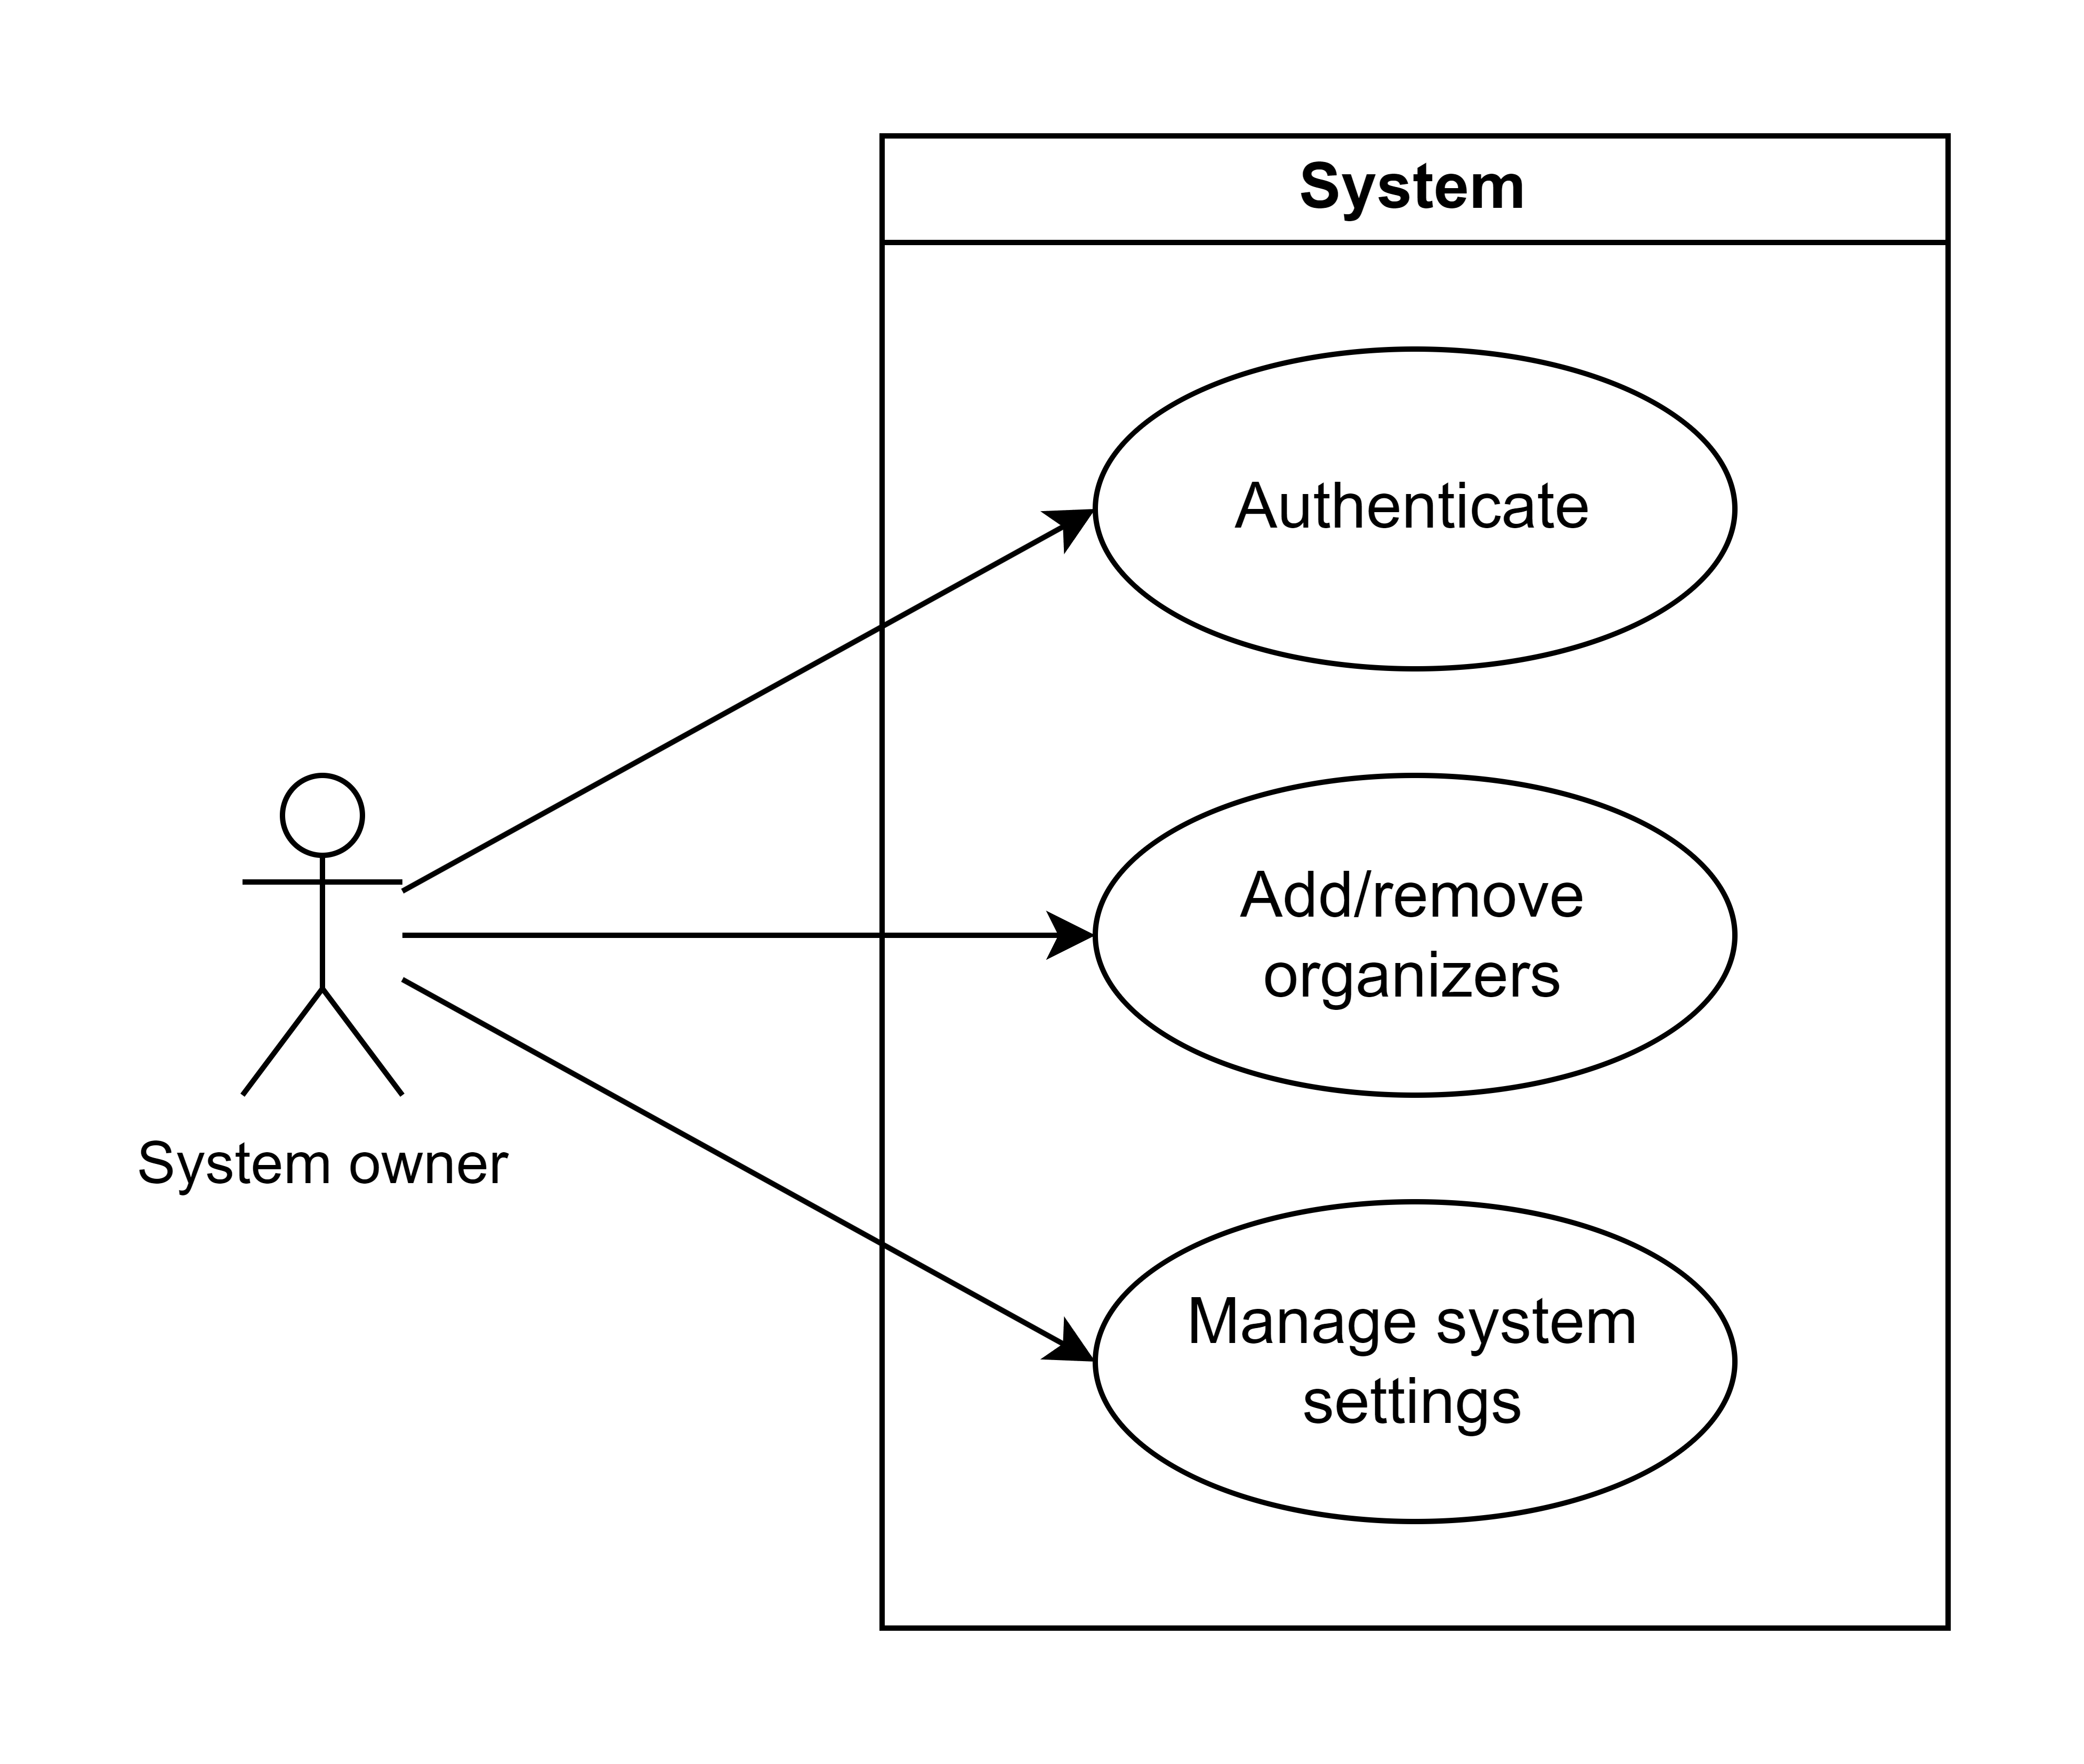
\includegraphics[width=\textwidth/2]{System owner use cases.png}
    \centering
    \caption{System owner use cases}
    \label{fig:system_owner_use_cases}
\end{figure}

\subsection{Organizer use cases}
\label{subsec:organizer_use_cases}

\begin{figure}[H]
    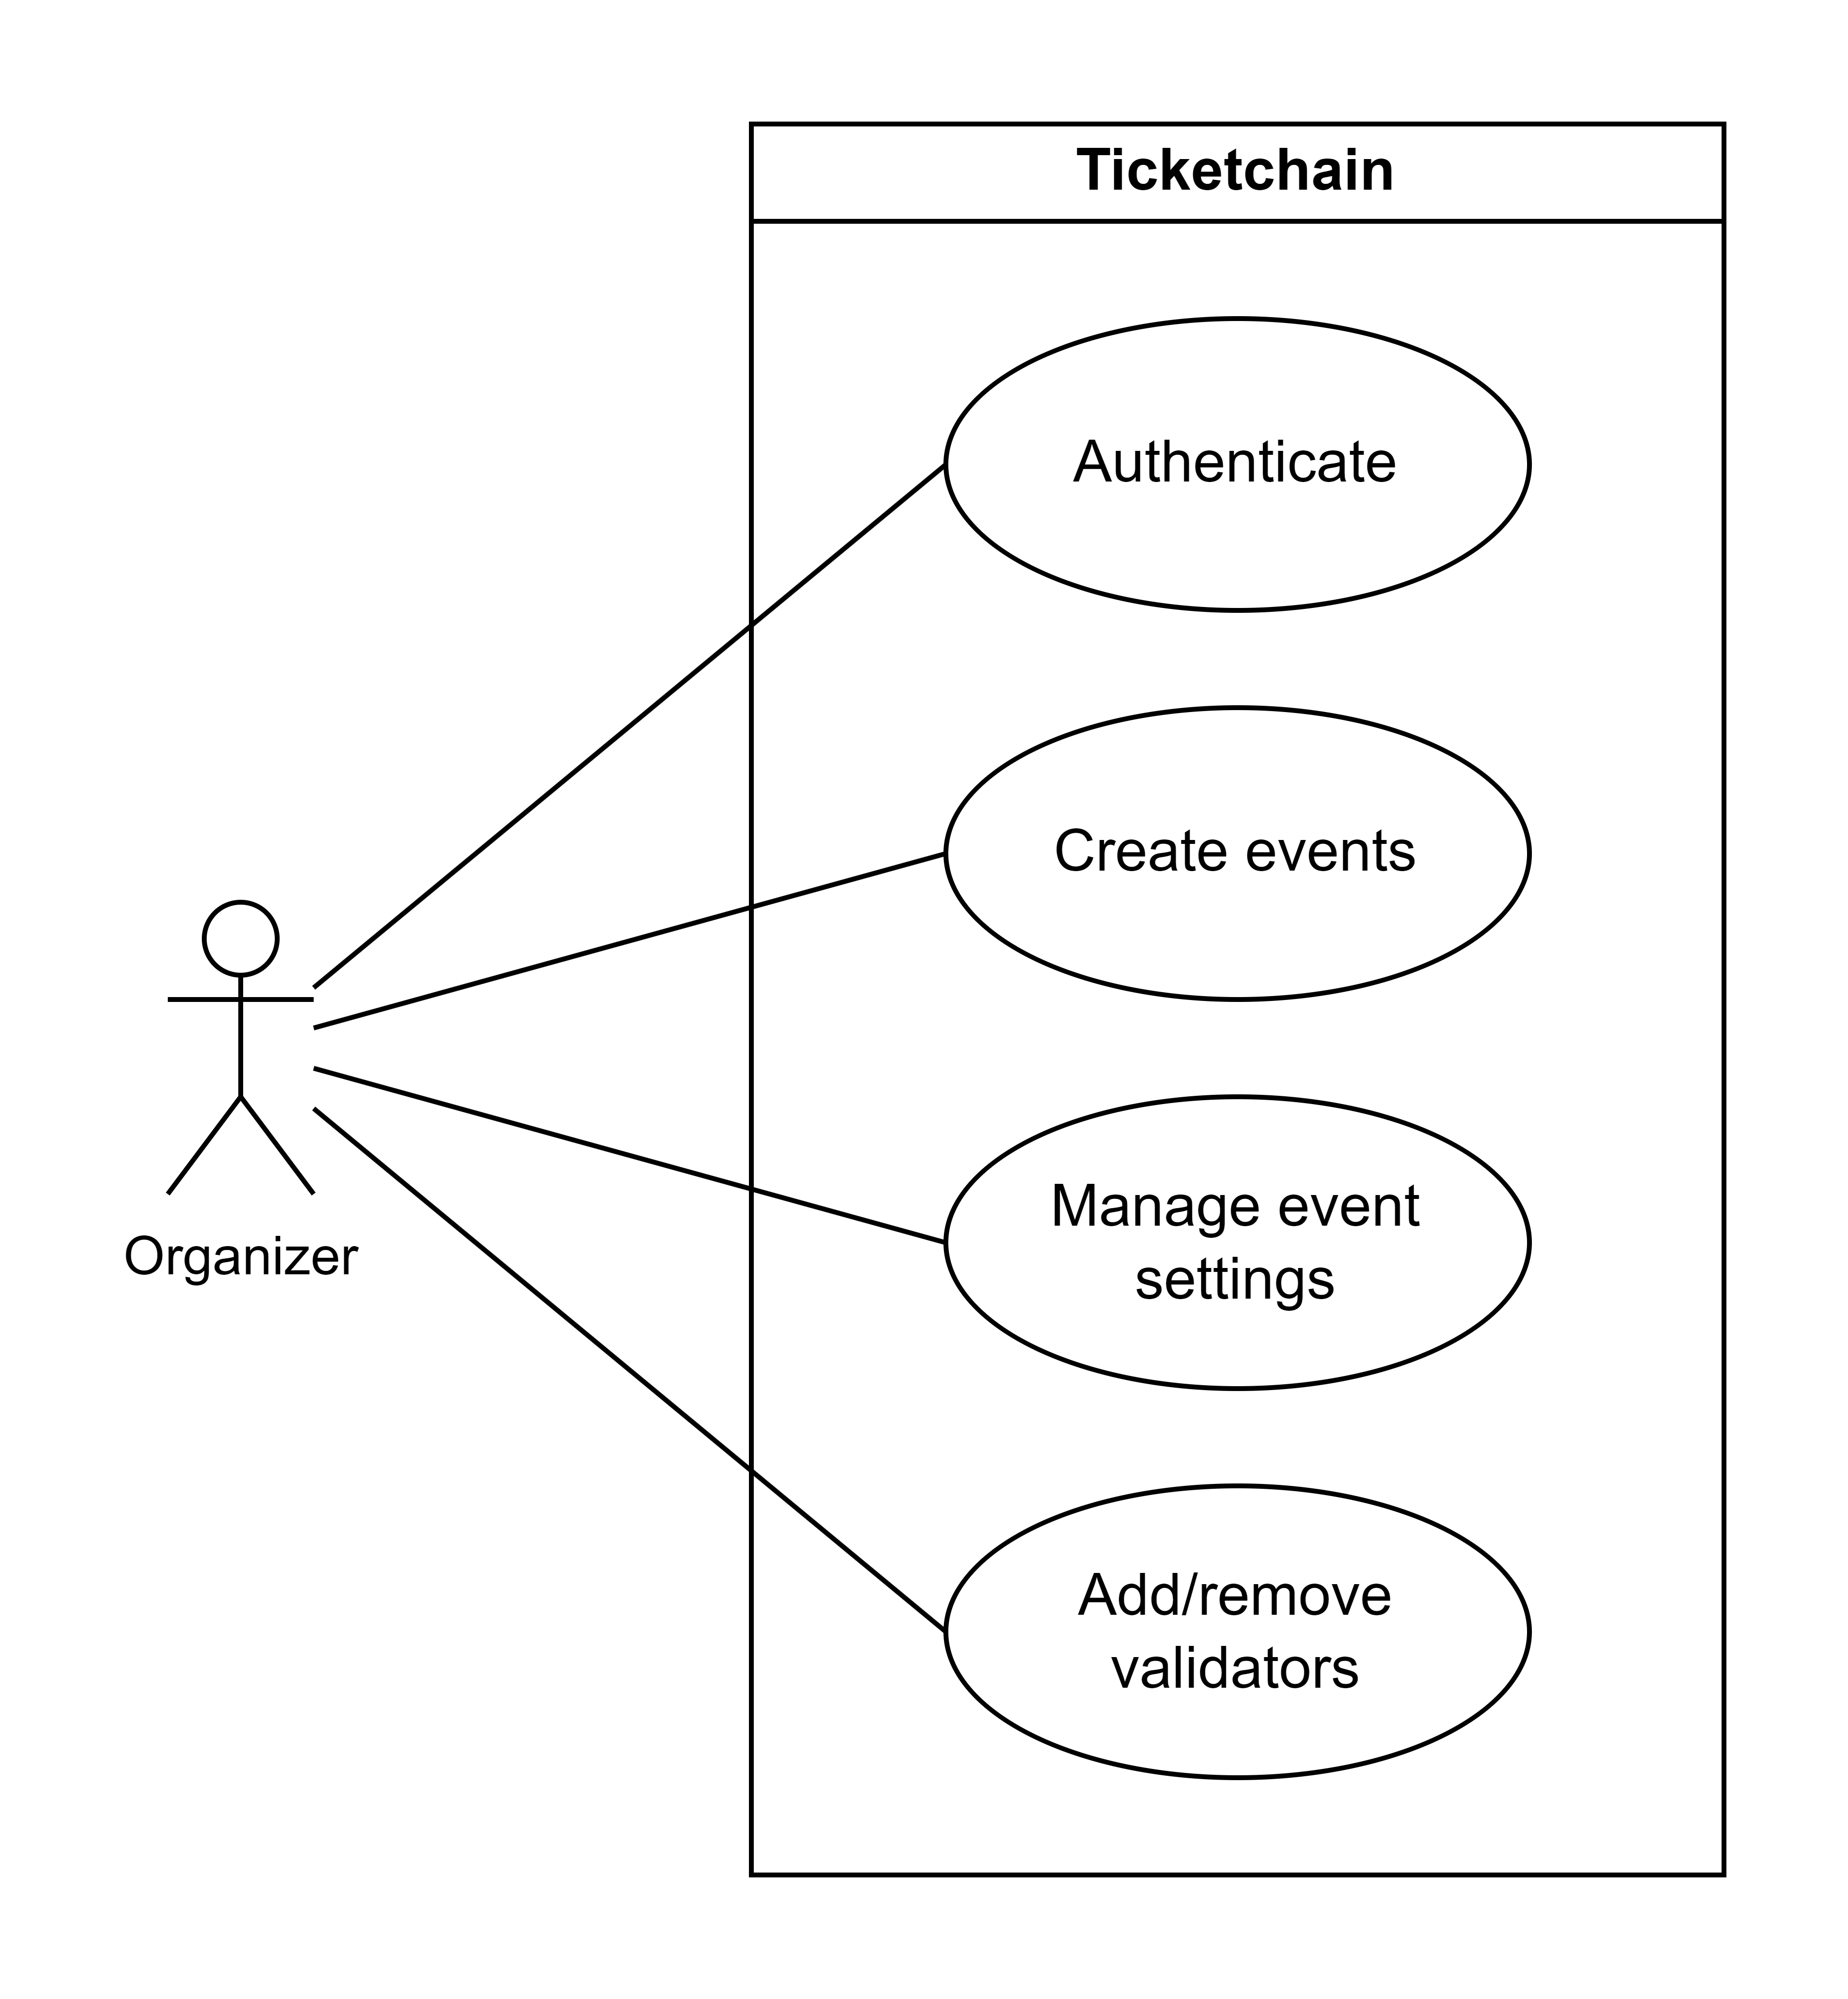
\includegraphics[width=\textwidth/2]{Organizer use cases.png}
    \centering
    \caption{Organizer use cases}
    \label{fig:organizer_use_cases}
\end{figure}

\subsection{Validator use cases}
\label{subsec:validator_use_cases}

\begin{figure}[H]
    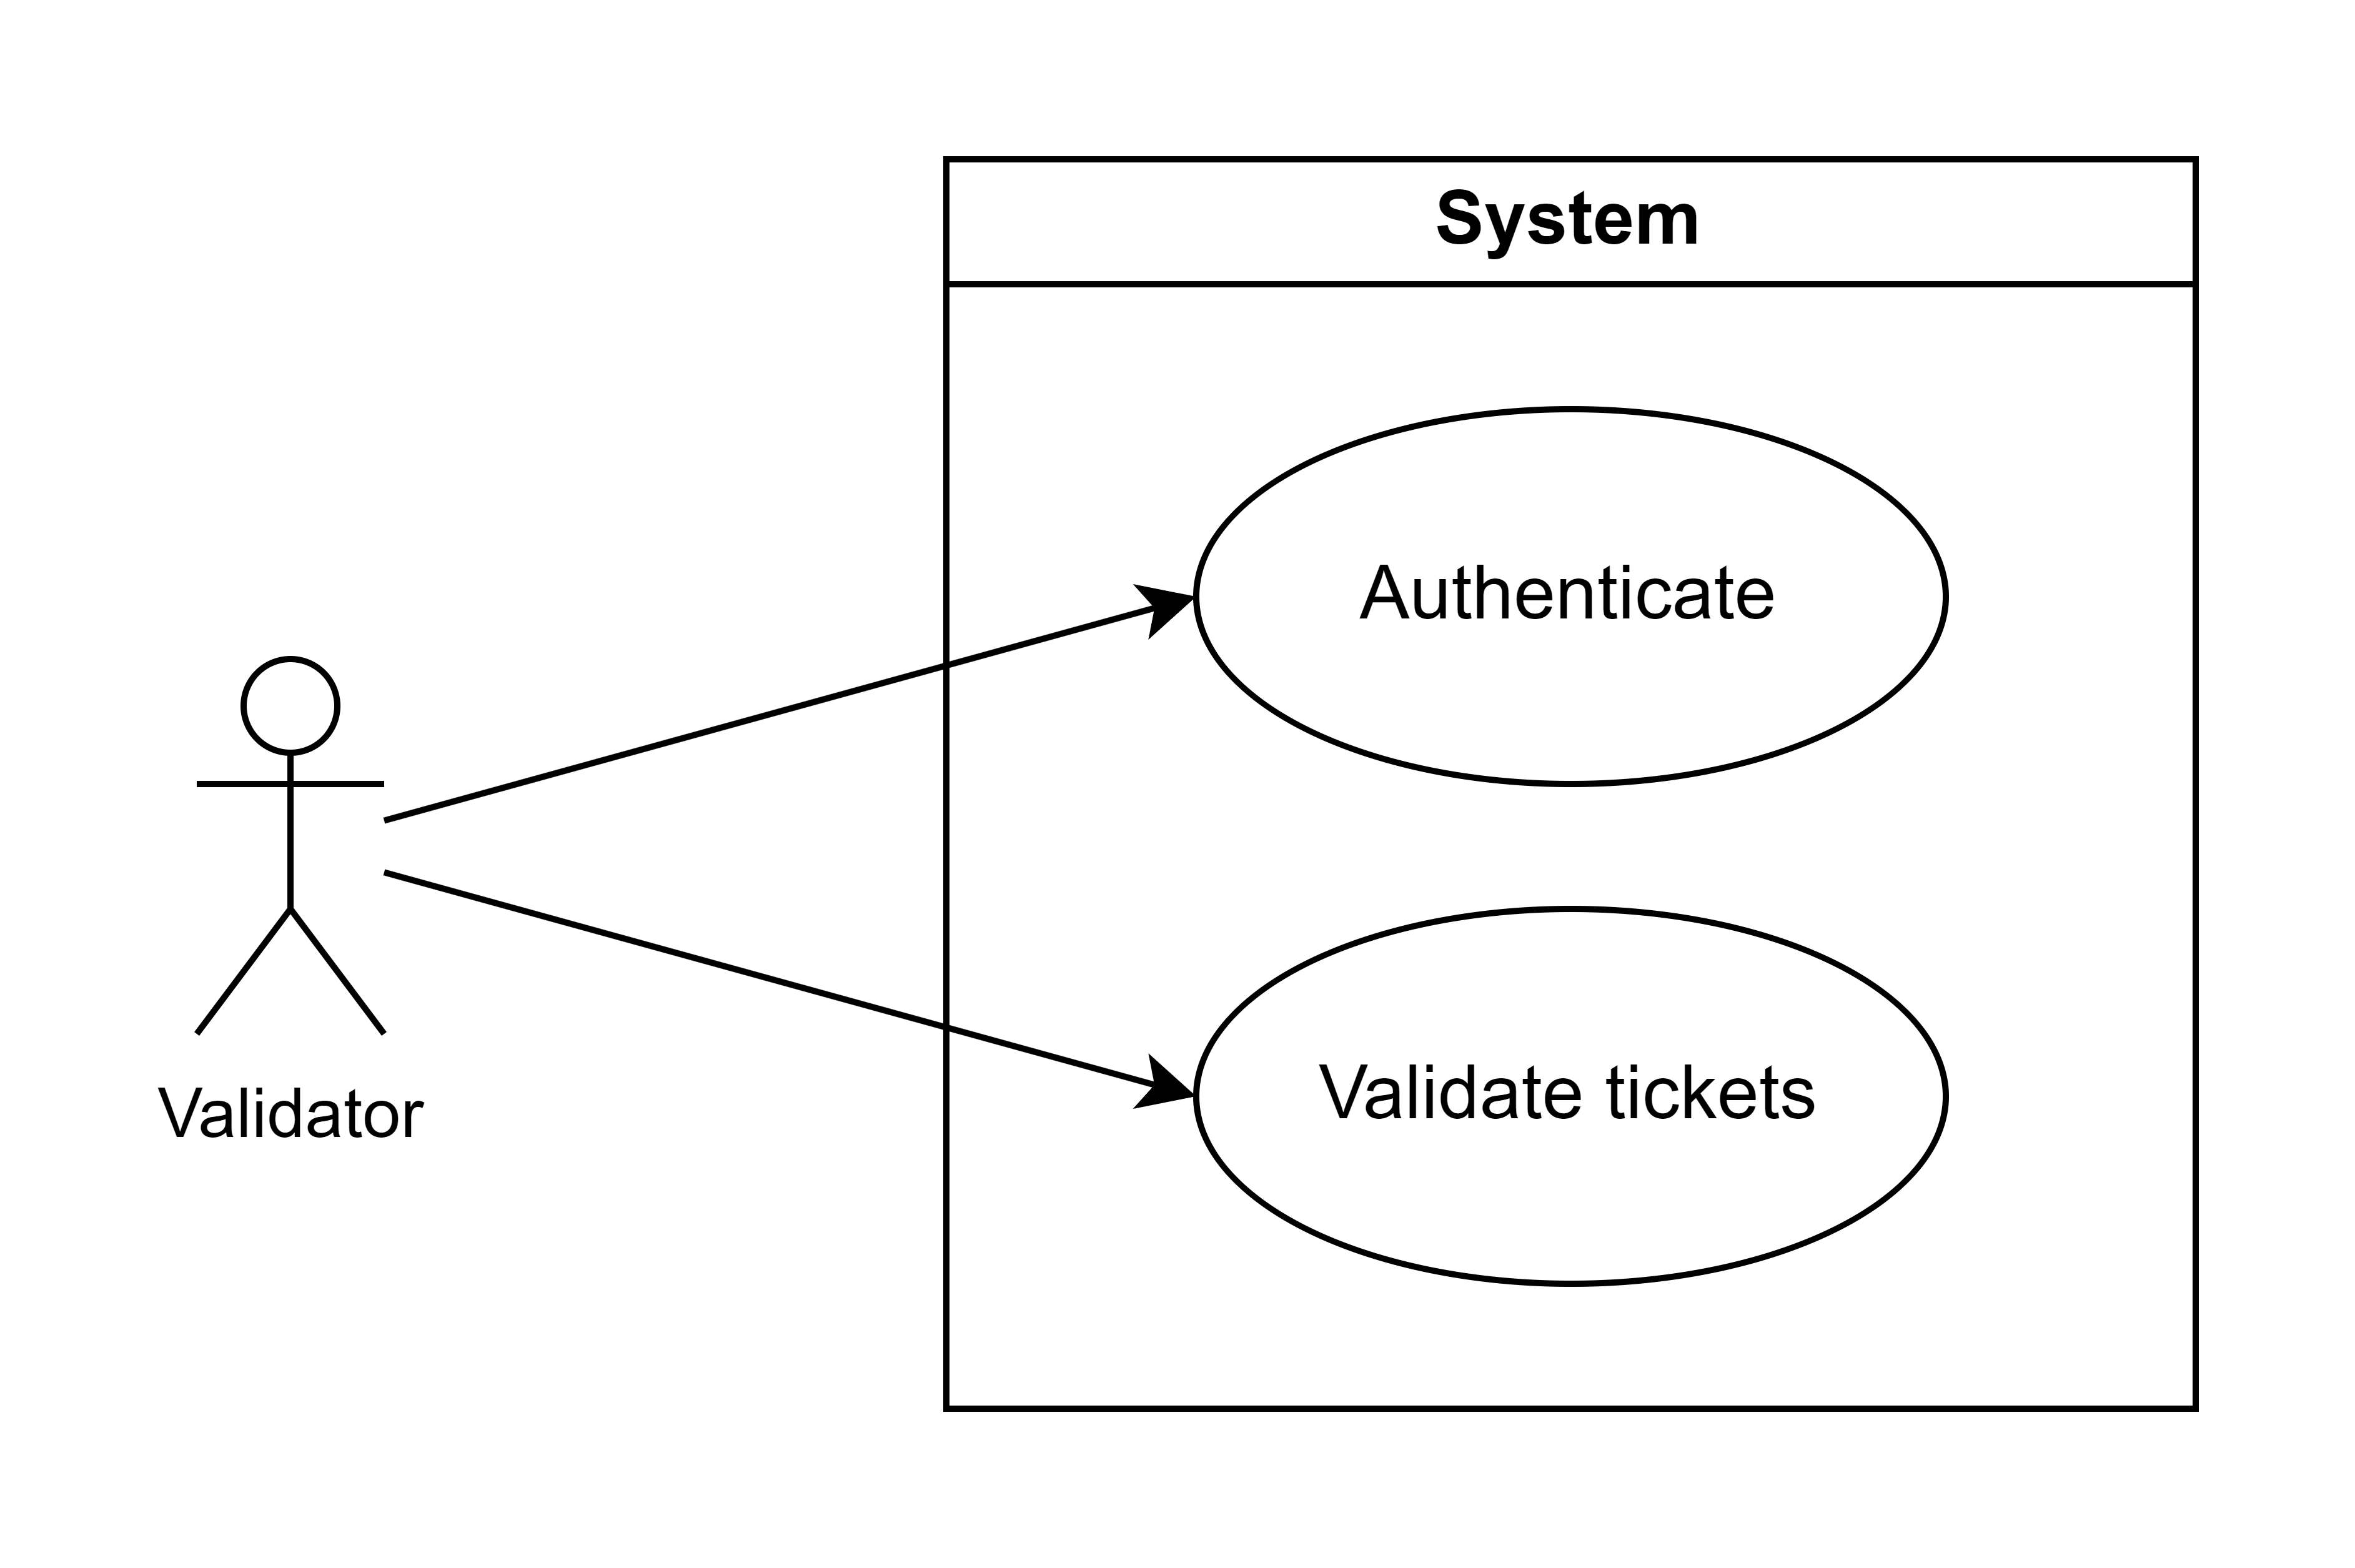
\includegraphics[width=\textwidth/2]{Validator use cases.png}
    \centering
    \caption{Validator use cases}
    \label{fig:validator_use_cases}
\end{figure}

\subsection{User use cases}
\label{subsec:user_use_cases}

\begin{figure}[H]
    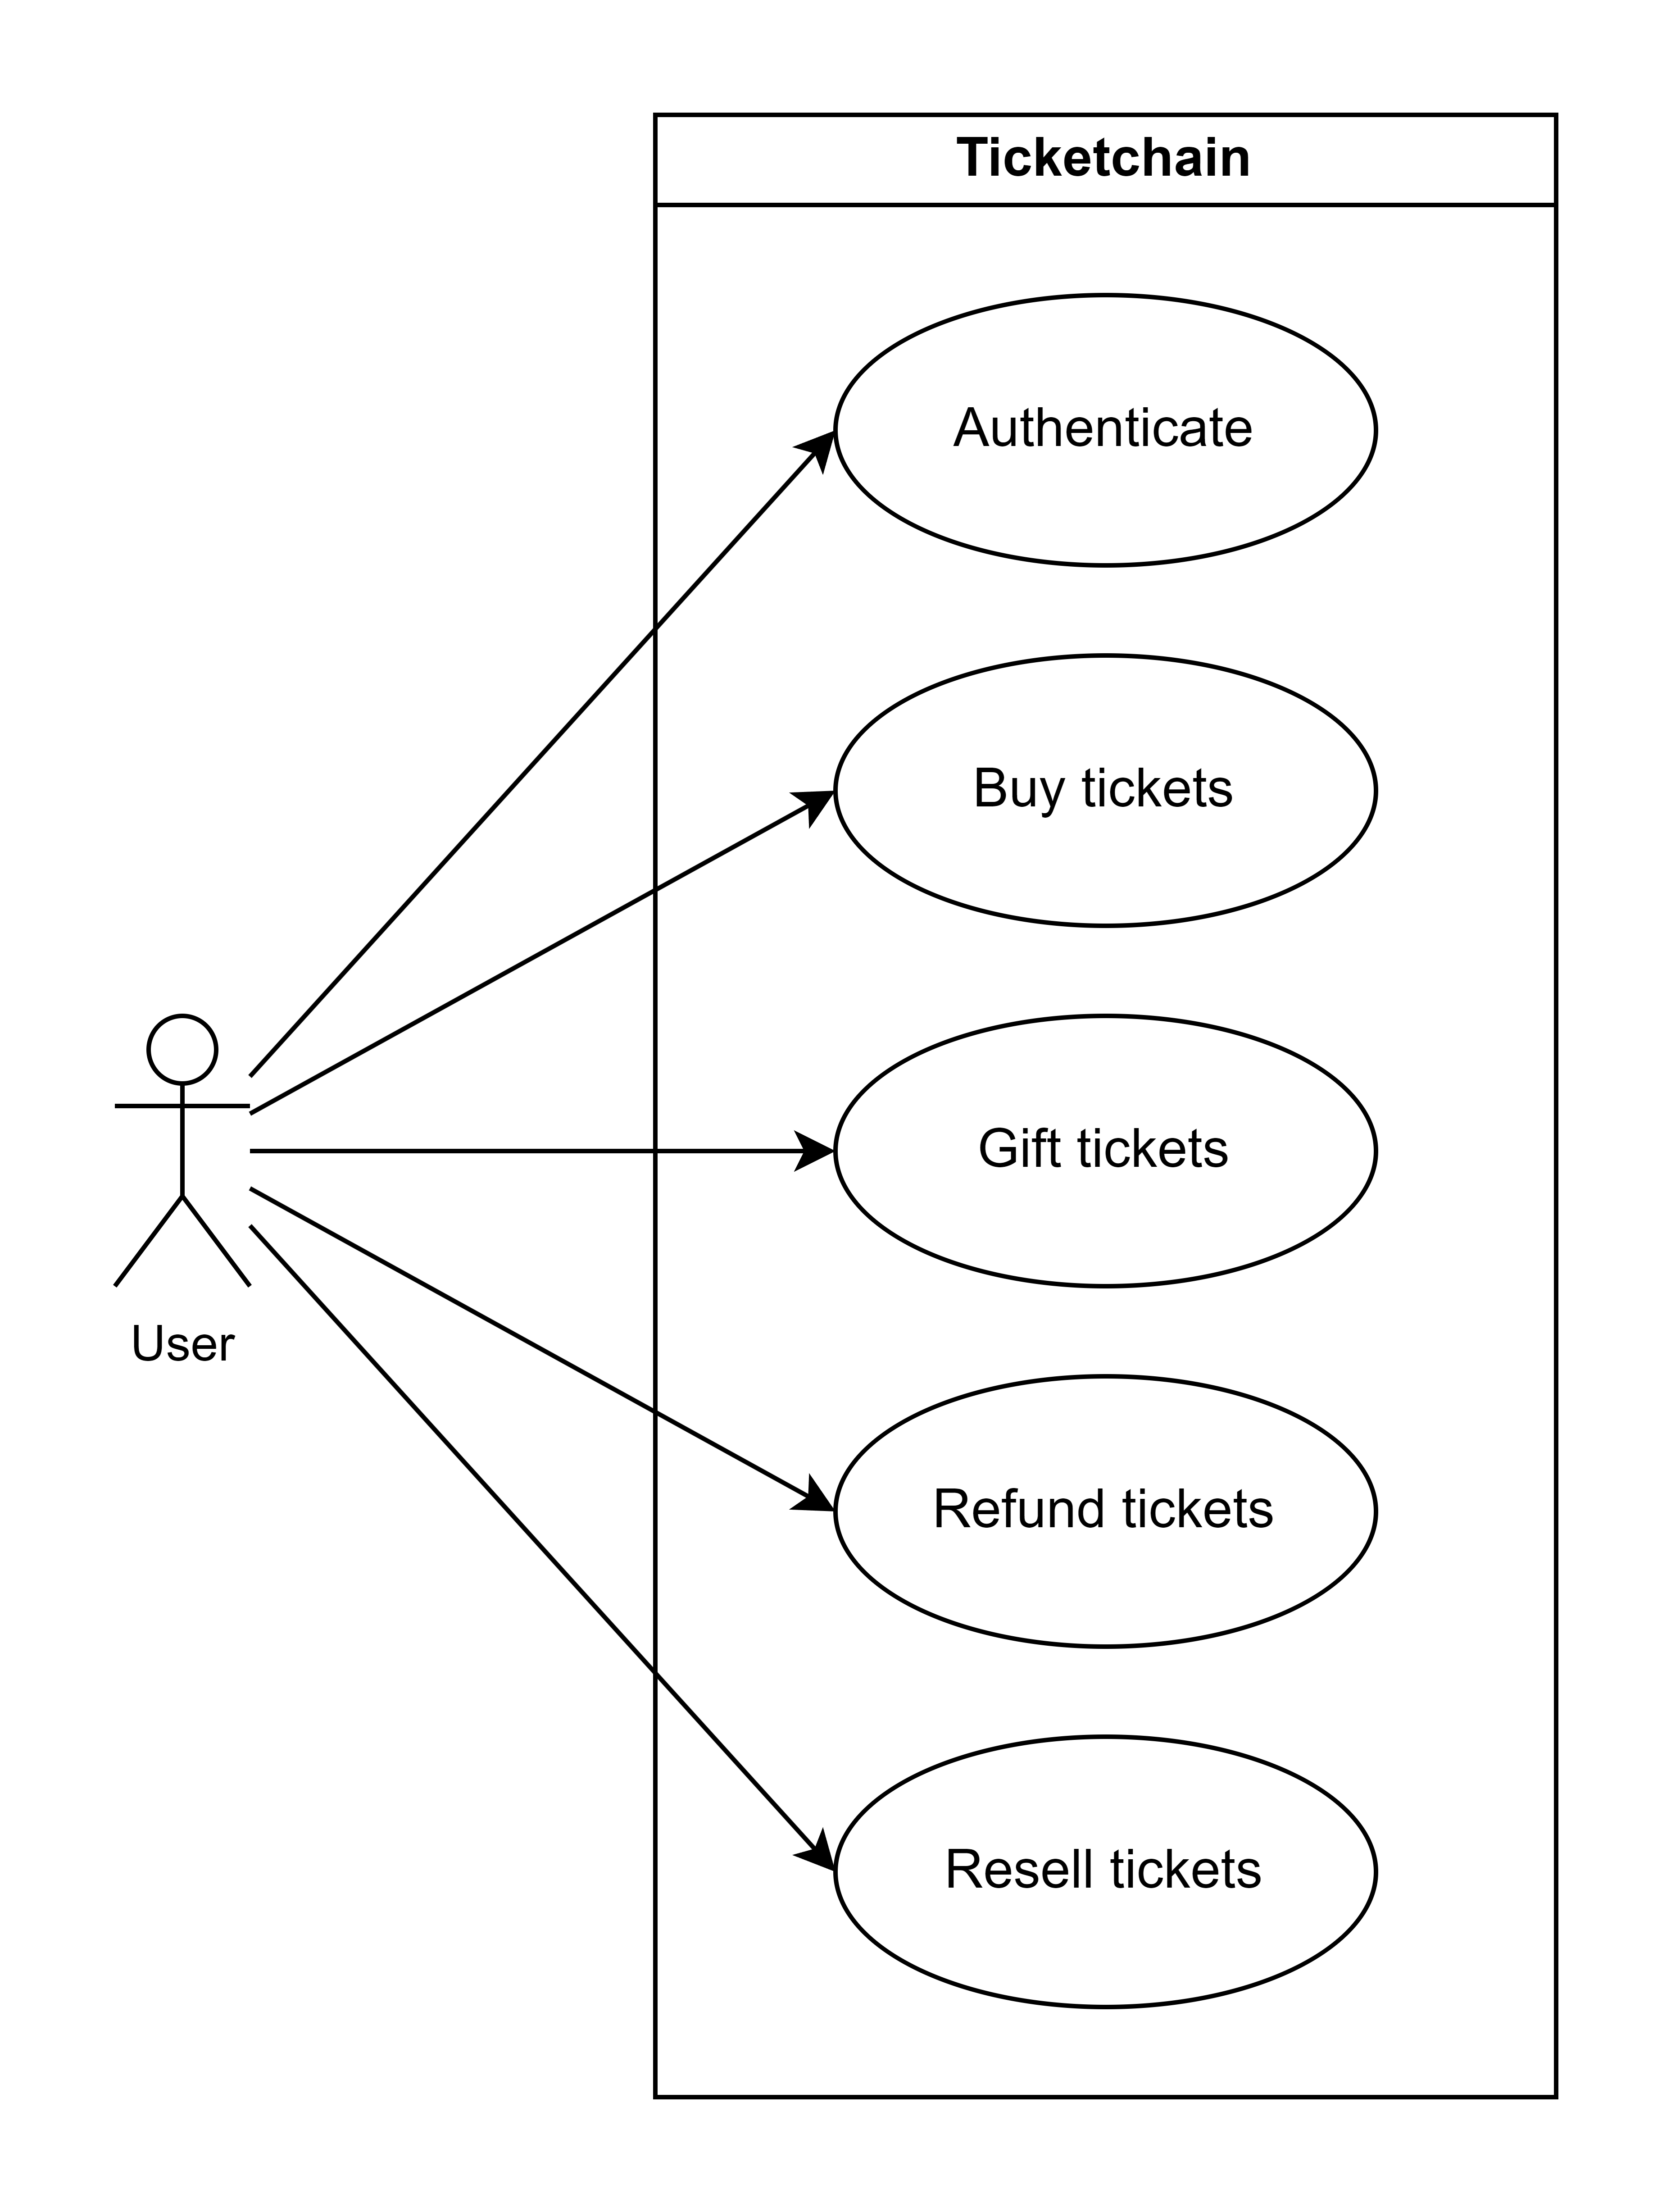
\includegraphics[width=\textwidth/2]{User use cases.png}
    \centering
    \caption{User use cases}
    \label{fig:user_use_cases}
\end{figure}
